% \section{Teaser}

 % \teaser{
 %   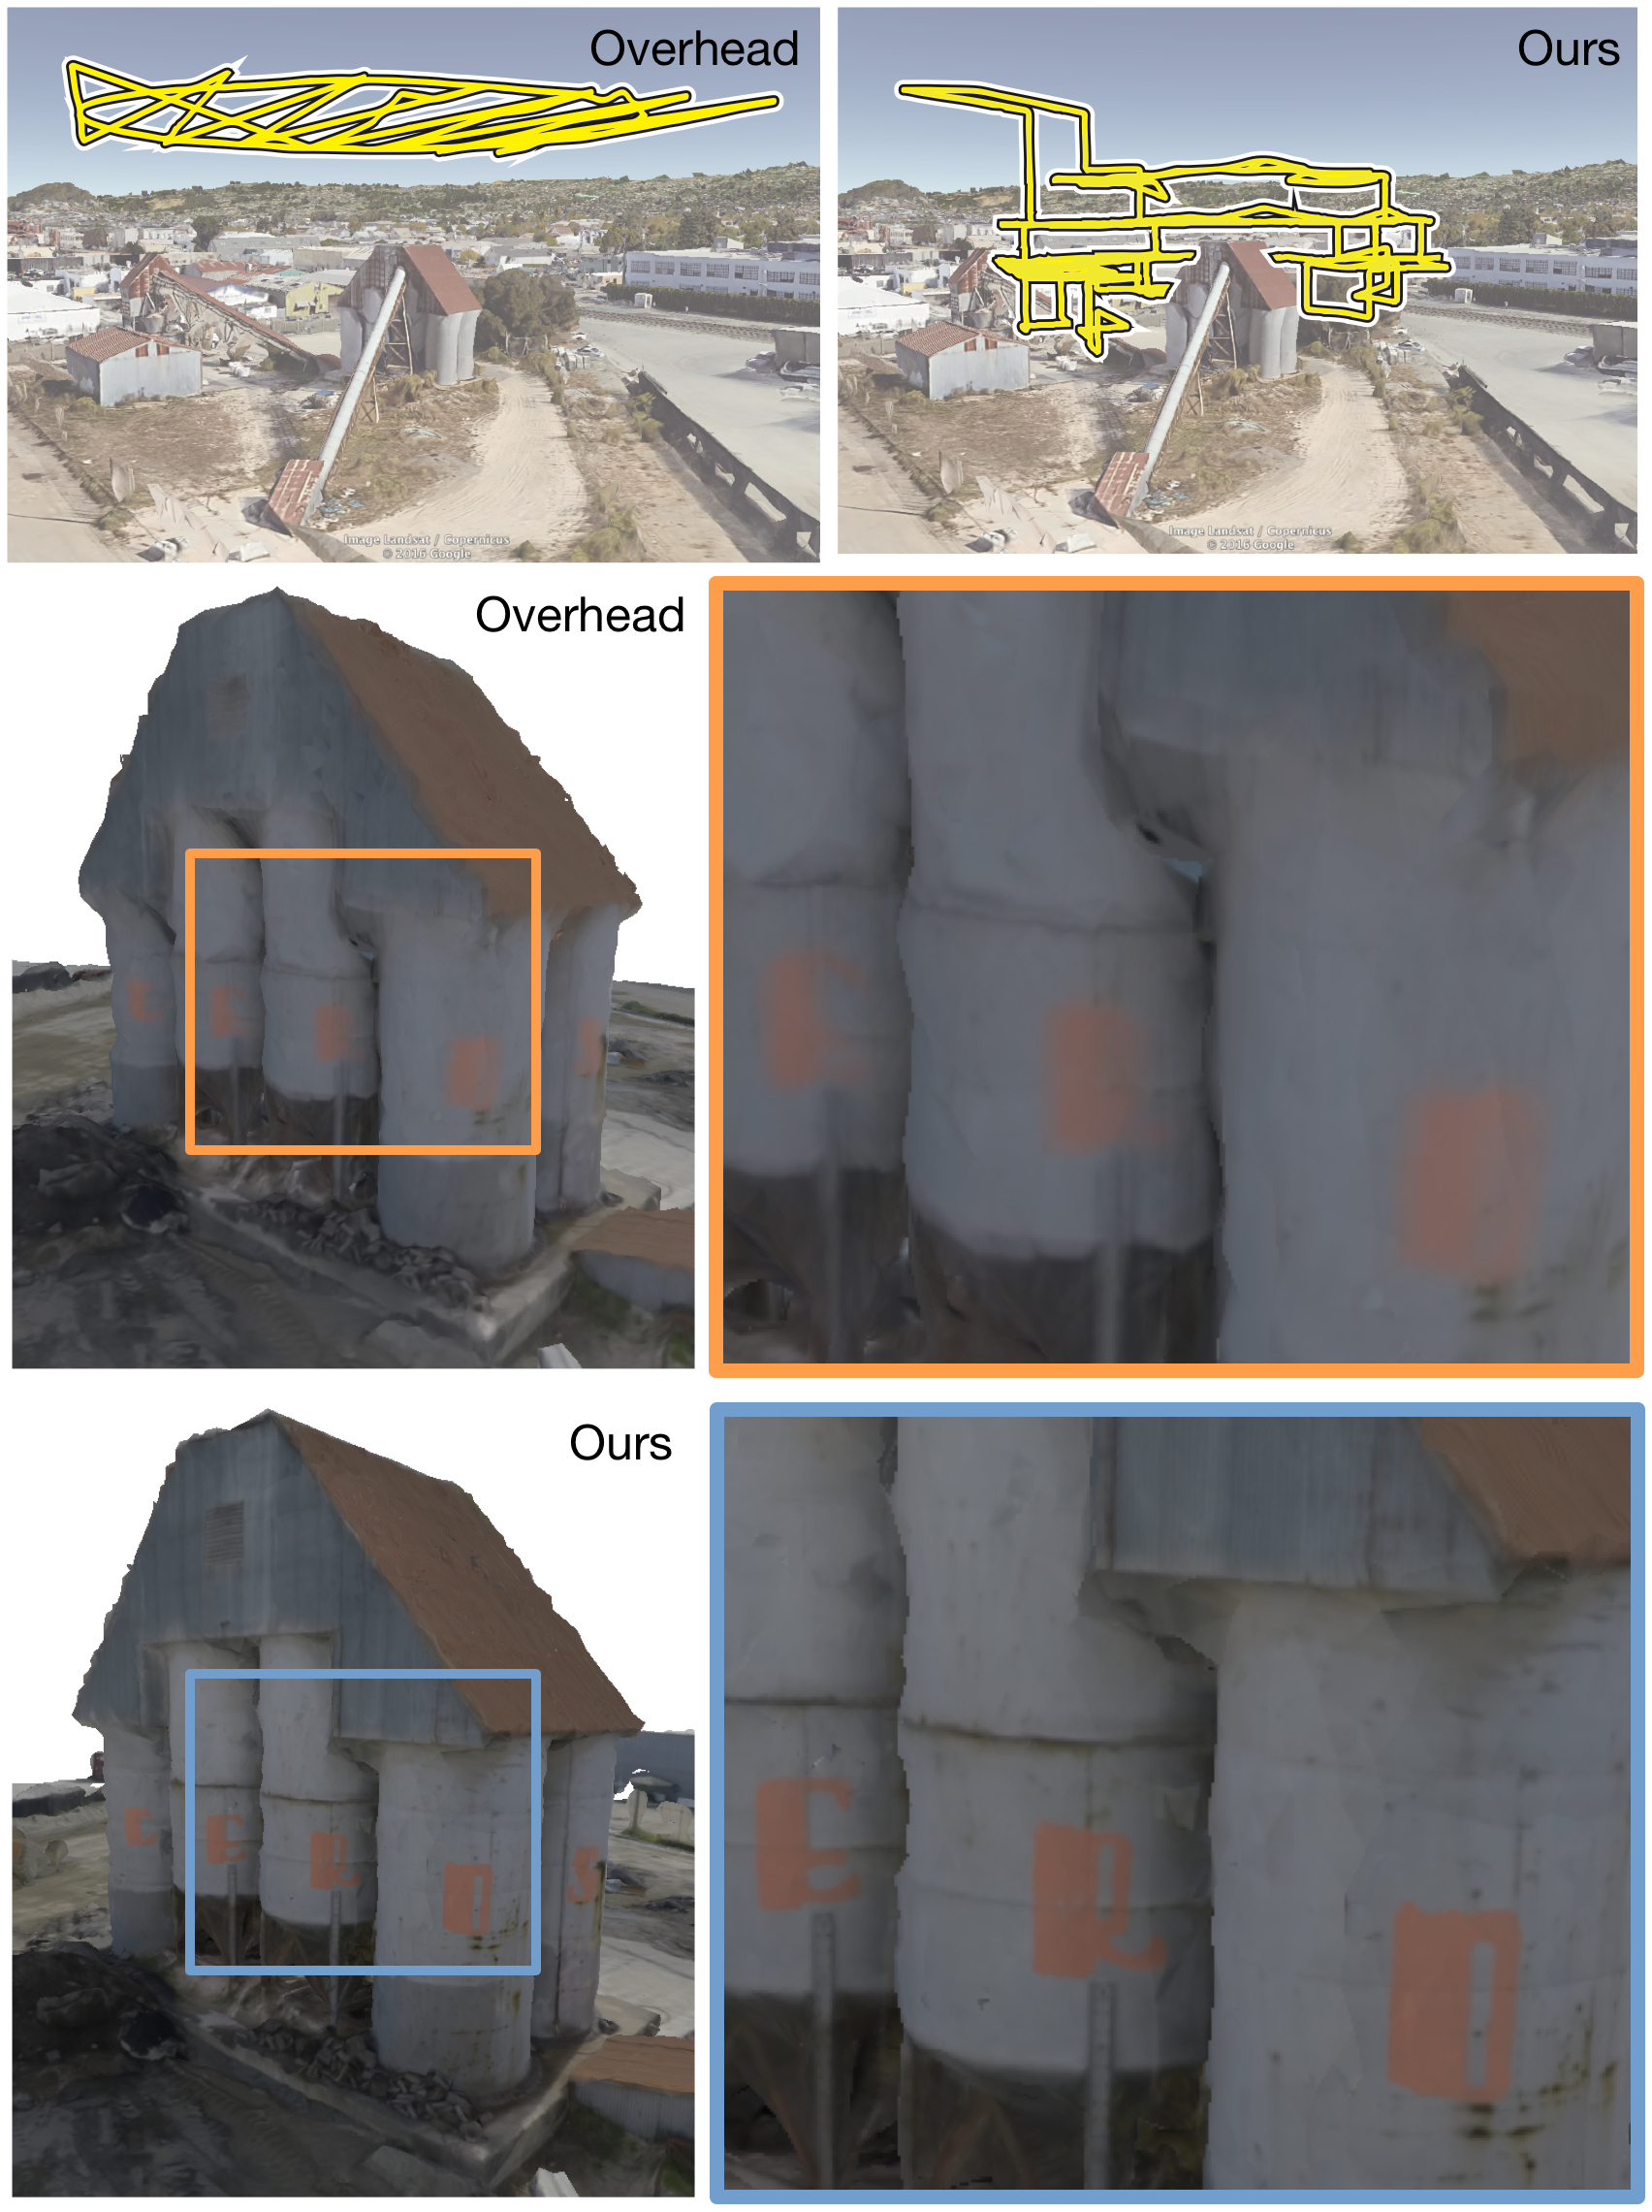
\includegraphics[width=7.0in]{images/teaser.pdf}

 %   \caption{
 %   (Left) Our interactive tool for designing quadrotor camera shots.
 %   In our tool, users specify camera pose keyframes in a virtual environment using a 3D scene view (a) and a 2D map view (b).
 %   Our tool synthesizes a camera trajectory that obeys the physical equations of motion for quadrotors, and interpolates between the user-specified keyframes.
 %   Users can preview the resulting shot in the virtual environment, using the playback buttons and scrubber interface to navigate through the shot (c).
 %   Users can also control the precise timing of the shot by editing easing curves (d).
 %   Users can set the virtual camera's field of view to match their real-world camera (e).
 %   Our tool provides the user with visual feedback about the physical feasibility of the resulting trajectory, notifying the user if her intended trajectory violates the physical limits of her quadrotor hardware (f).
 %   Once the user is satisfied with her shot, she presses the Start Capture button (g).
 %   (Right) Our tool commands a quadrotor camera to execute the resulting trajectory fully autonomously, capturing real video footage that is faithful to the virtual preview.
 %   We show frames from our real-world video output, with corresponding frames from the virtual preview shown as small insets (h).
 %   }
 %   \label{fig:teaser}
 % }

